\documentclass[a4paper]{article}
\usepackage[utf8]{inputenc}

\usepackage{graphicx}
\usepackage{booktabs}
\usepackage{subfig}

\usepackage[danish]{babel}
\usepackage{mathpazo}
\renewcommand{\danishhyphenmins}{22} % bedre orddeling
\usepackage[T1]{fontenc}
\usepackage{amsmath,amssymb}

\usepackage{fancyhdr}
\pagestyle{fancy}
\lhead{}\chead{}\rhead{Københavns Universitet}
\lfoot{}\cfoot{\thepage}\rfoot{}

\title{}
\author{Claus Skou Nielsen, Michael Budde, Kasper Passov, Niels Ørbæk
Christensen}
\begin{document}
\section{Arbejdsopgaver}
Vi har udført følgende arbejdsopgaver:
\begin{itemize}
\item{\textbf{Opgave 1:}}
    Undersøg prisen for en ford transit fra København til Fyn
\item{\textbf{Opgave 2:}}
    Bestil en varevogn fra København til Fyn
\item{\textbf{Opgave 3:}}
    Ændre returpunktet fra Fyn til Jylland
\item{\textbf{Opgave 4:}}
    Slet bestilingen
\end{itemize}

\section{Elementer i brugergrænsefladen}
\subsection{Fokus på brugerens opgaver}
De har en brugercentreret forside, fordi de har valgt at have
reservationsformularen på forsiden. Det hovedsalige formål for brugere af siden,
er at reservere/leje biler, og derfor giver det god mening at give netop denne
funktionalitet meget synlighed. I det aspekt er der fokus på brugerens opgaver
(Figur \ref{forside}).

\begin{figure}[htbp]
  \begin{center}
    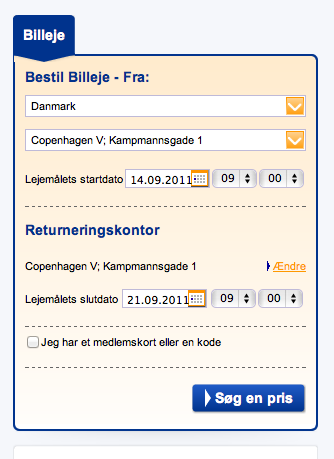
\includegraphics[scale=.6]{1.png}
  \end{center}
  \caption{Forside, reservationsformular.}
  \label{forside}
\end{figure}

En anden opgave en bruger kan have, er muligheden for at annullere en ordre. På
dette punkt har siden gemt funktionaliteten væk i en underside, der ikke giver
mening Figur \ref{annullering}.

\begin{figure}[htbp]
  \begin{center}
    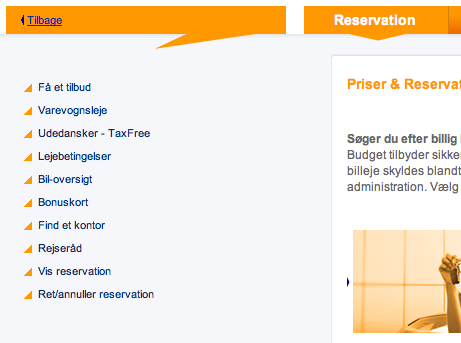
\includegraphics[scale=.6]{3.png}
  \end{center}
  \caption{Annullering af ordre gemt væk.}
  \label{annullering}
\end{figure}

\subsection{Synlighed på systemets status}
Systemets status er relevant når siden henter informationer til brugeren. Når
applikationen finder ledige biler frem, vises systemets status mens der bliver
hentet information. Det opfylder kravet om synlighed Figur \ref{status}.

\begin{figure}[htbp]
  \begin{center}
    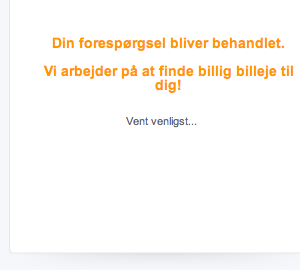
\includegraphics[scale=.6]{4.png}
  \end{center}
  \caption{Systemets status.}
  \label{status}
\end{figure}
\subsection{Match between system and the real world}
Siden bruger ikke komplicerede eller tekniske termer til at beskrive bilerne man
kan leje, men holder derimod sproget i menigmandszonen (Figur \ref{sprog}).

\begin{figure}[htbp]
  \begin{center}
    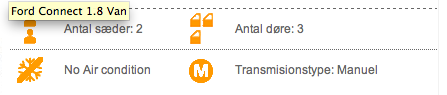
\includegraphics[scale=.6]{5.png}
  \end{center}
  \caption{Sproget er i menigmandszonen.}
  \label{sprog}
\end{figure}

Siden viser menupunkter og information i en naturlig orden, hvor det vigtigste
for brugeren bliver vist først. Se Figur \ref{menu}.

\begin{figure}[htbp]
  \begin{center}
    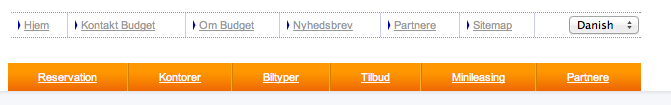
\includegraphics[width=\textwidth]{2.png}
  \end{center}
  \caption{Menupunkter.}
  \label{menu}
\end{figure}

\subsection{Brugerens kontrol og frihed}
Der er god mulighed for at hoppe frem og tilbage i forskellige stadier af
reservationen. Det er også muligt at slette reservationen når den er blevet
oprettet (Figur \ref{stadier}).

Stadieoversigten kan dog være svær at få øje på.
\begin{figure}[htbp]
  \begin{center}
    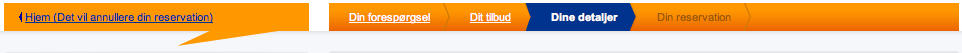
\includegraphics[width=\textwidth]{9.png}
  \end{center}
  \caption{Forskellige stadier af bestillingsprocessen.}
  \label{stadier}
\end{figure}

\subsection{Consistency and standards}
Vi har ikke været i stand til at finde handlinger, ord eller situationer der
betyder det samme og forvirrer brugerne.

\subsection{Error prevention}
Hvis man indtaster en afleveringsdato der er tidligere end afhentningsdatoen,
kommer siden med to fejlmeddelelser, hvilket ikke er videre elegant (se Figur
\ref{fejl_datoer}).

\begin{figure}[htbp]
  \begin{center}
    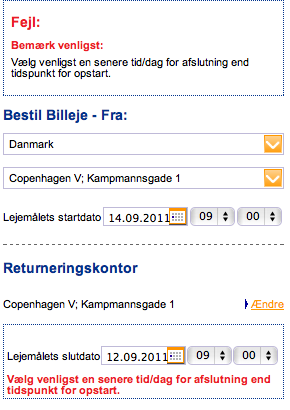
\includegraphics[scale=.6]{6.png}
  \end{center}
  \caption{Fejlmeddelelse ved forkert indtastning af datoer.}
  \label{fejl_datoer}
\end{figure}

Når man indtaster kontaktinformation forkert, viser siden de fejlagtige
indtastninger korrekt (Figur \ref{fejl_boks} og \ref{fejl_kontaktinformation})

\begin{figure}[htbp]
  \begin{center}
    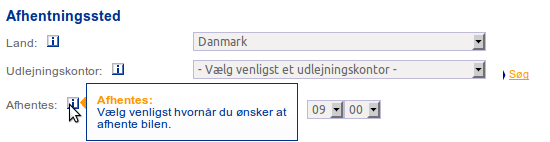
\includegraphics[scale=.6]{7.png}
  \end{center}
  \caption{Fejlboks ved forkert indtastning af kontaktinformation.}
  \label{fejl_boks}
\end{figure}

\begin{figure}[htbp]
  \begin{center}
    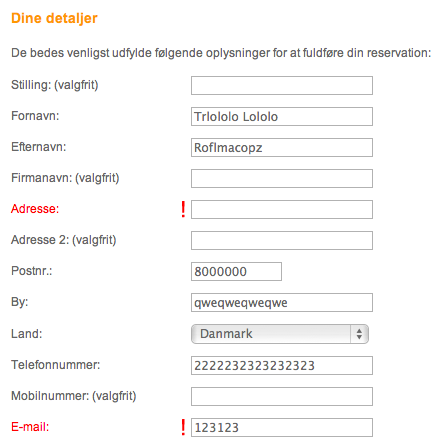
\includegraphics[scale=.6]{8.png}
  \end{center}
  \caption{Fejlmeddelelser ved forkert indtastning af kontaktinformation.}
  \label{fejl_kontaktinformation}
\end{figure}

\subsection{Brugerinput huskes}
Siden husker indtastede data på tværs af stadier. Brugeren bliver ikke tvunget
til selv at huske noget.

Der er hjælpeknapper, og de handlinger hvis betydning ikke er indlysende har en
forklaring

\subsection{Fleksibilitet og effektivitet}
Der er ikke mulighed for at lagre sin kontaktinformation på siden, ved fx at
oprette en bruger.

Det er heller ikke muligt at bruge en tidligere reservering. Man kunne
forestille sig en bruger, der jævnligt lejer den samme bil, fra det samme
afhentningssted og afleverer den ved det samme afleveringssted.

\subsection{Æstetik og minimalistisk design}
De holder et stabilt farveskema (læs: orange og blåt) igennem alle sidens
undersider og funktioner. Siden er ikke videre køn, og der bliver brugt meget
plads på forsiden til reklame for firmaet, hvilket ikke er minimalistisk.

I bestillingsproceduren er reklamerne fjernet, og derfor opfylder de kravene om
et minimalistisk design, selv om sidens design ligner noget fra et andet
årtusinde.
\end{document}
